\documentclass[]{article}
\usepackage[T1]{fontenc}
\usepackage[utf8]{inputenc}
%\usepackage[icelandic]{babel}
\usepackage{caption}
\usepackage{circuitikz}
\usepackage{grffile} 
\usepackage[margin=1in]{geometry}
\usepackage{listings}
\usepackage{amsmath,amsfonts,amssymb}
\usepackage{tikz}
\usetikzlibrary{automata,positioning}
% trees
\usepackage[]{forest}
\forestset{.style={for tree=
{parent anchor=south, child anchor=north,align=center,inner sep=2pt}}}
%fyrir listing
\lstset{
  basicstyle=\itshape,
  xleftmargin=3em,
  literate={->}{$\rightarrow$}{2}
           {α}{$\alpha$}{1}
           {δ}{$\delta$}{1}
           {eps}{$\epsilon$}{3}
           {|}{$\vert$}{1}
}

% grffile er pakki sem leifir manni að nota "" til þess að forðast að nota
% nafnið á myndinni með.
\usepackage{graphicx}
% \graphicspath{{images/}} Sýnir undir möppu þar sem myndirnar eru

\usepackage{hyperref}
%fyrirlinka - \url{www.....}
\begin{document}


\title{Formleg mál og reiknanleiki}
\author{Pétur}
\maketitle

\section*{1.}

\begin{tabular}{lll}
$q_{1}000$ 			& $\delta(q_{1},0)$ 	& = ($q_{2}$,$\sqcup$,R) \\
$\sqcup q_{2}00$ 	& $\delta(q_{2},0)$ 	& = ($q_{3}$,x,R) \\
$\sqcup xq_{3}0$ 	& $\delta(q_{3},0)$ 	& = ($q_{4}$,R) \\
$\sqcup x0q_{4}$ 	& $\delta(q_{4},\sqcup)$& = ($q_{reject}$,R) \\
\end{tabular}

\section*{2.}

\begin{lstlisting}
Input string w

while true do
	Sweep left to right across the tape, cross one a , b and c
	if single a left
		return accept
	else if single b left
		return accept
	else if single c left
		return accept
	else if a equals b or b equals c or c equals a
		return reject
\end{lstlisting}
\section*{3.}

\begin{lstlisting}
Input string w
while true do
	Sweep left to right across the tape. Mark x for 1 or 0
	closest to the beginning of the string then pass # and 
	mark x 	for 0 or 1 only if it equal the previous marked
	symbol closest to # on the right hand side. Then pas the 
	# on the right hand side and mark the next 0 or 1 only if 
	it equals the previous marked symbol.
	if only # and x
		return accept
	else if symbol 1 ... # .... n - i # .... n + i
	1 dose not equal n - i and 1 dose not equal n + i
		return reject
		// # n length #	i length
		// n + i = the length of the string
\end{lstlisting}

\pagebreak

\section*{4.}
The picture shows that the Language is Turing-recognizable\\


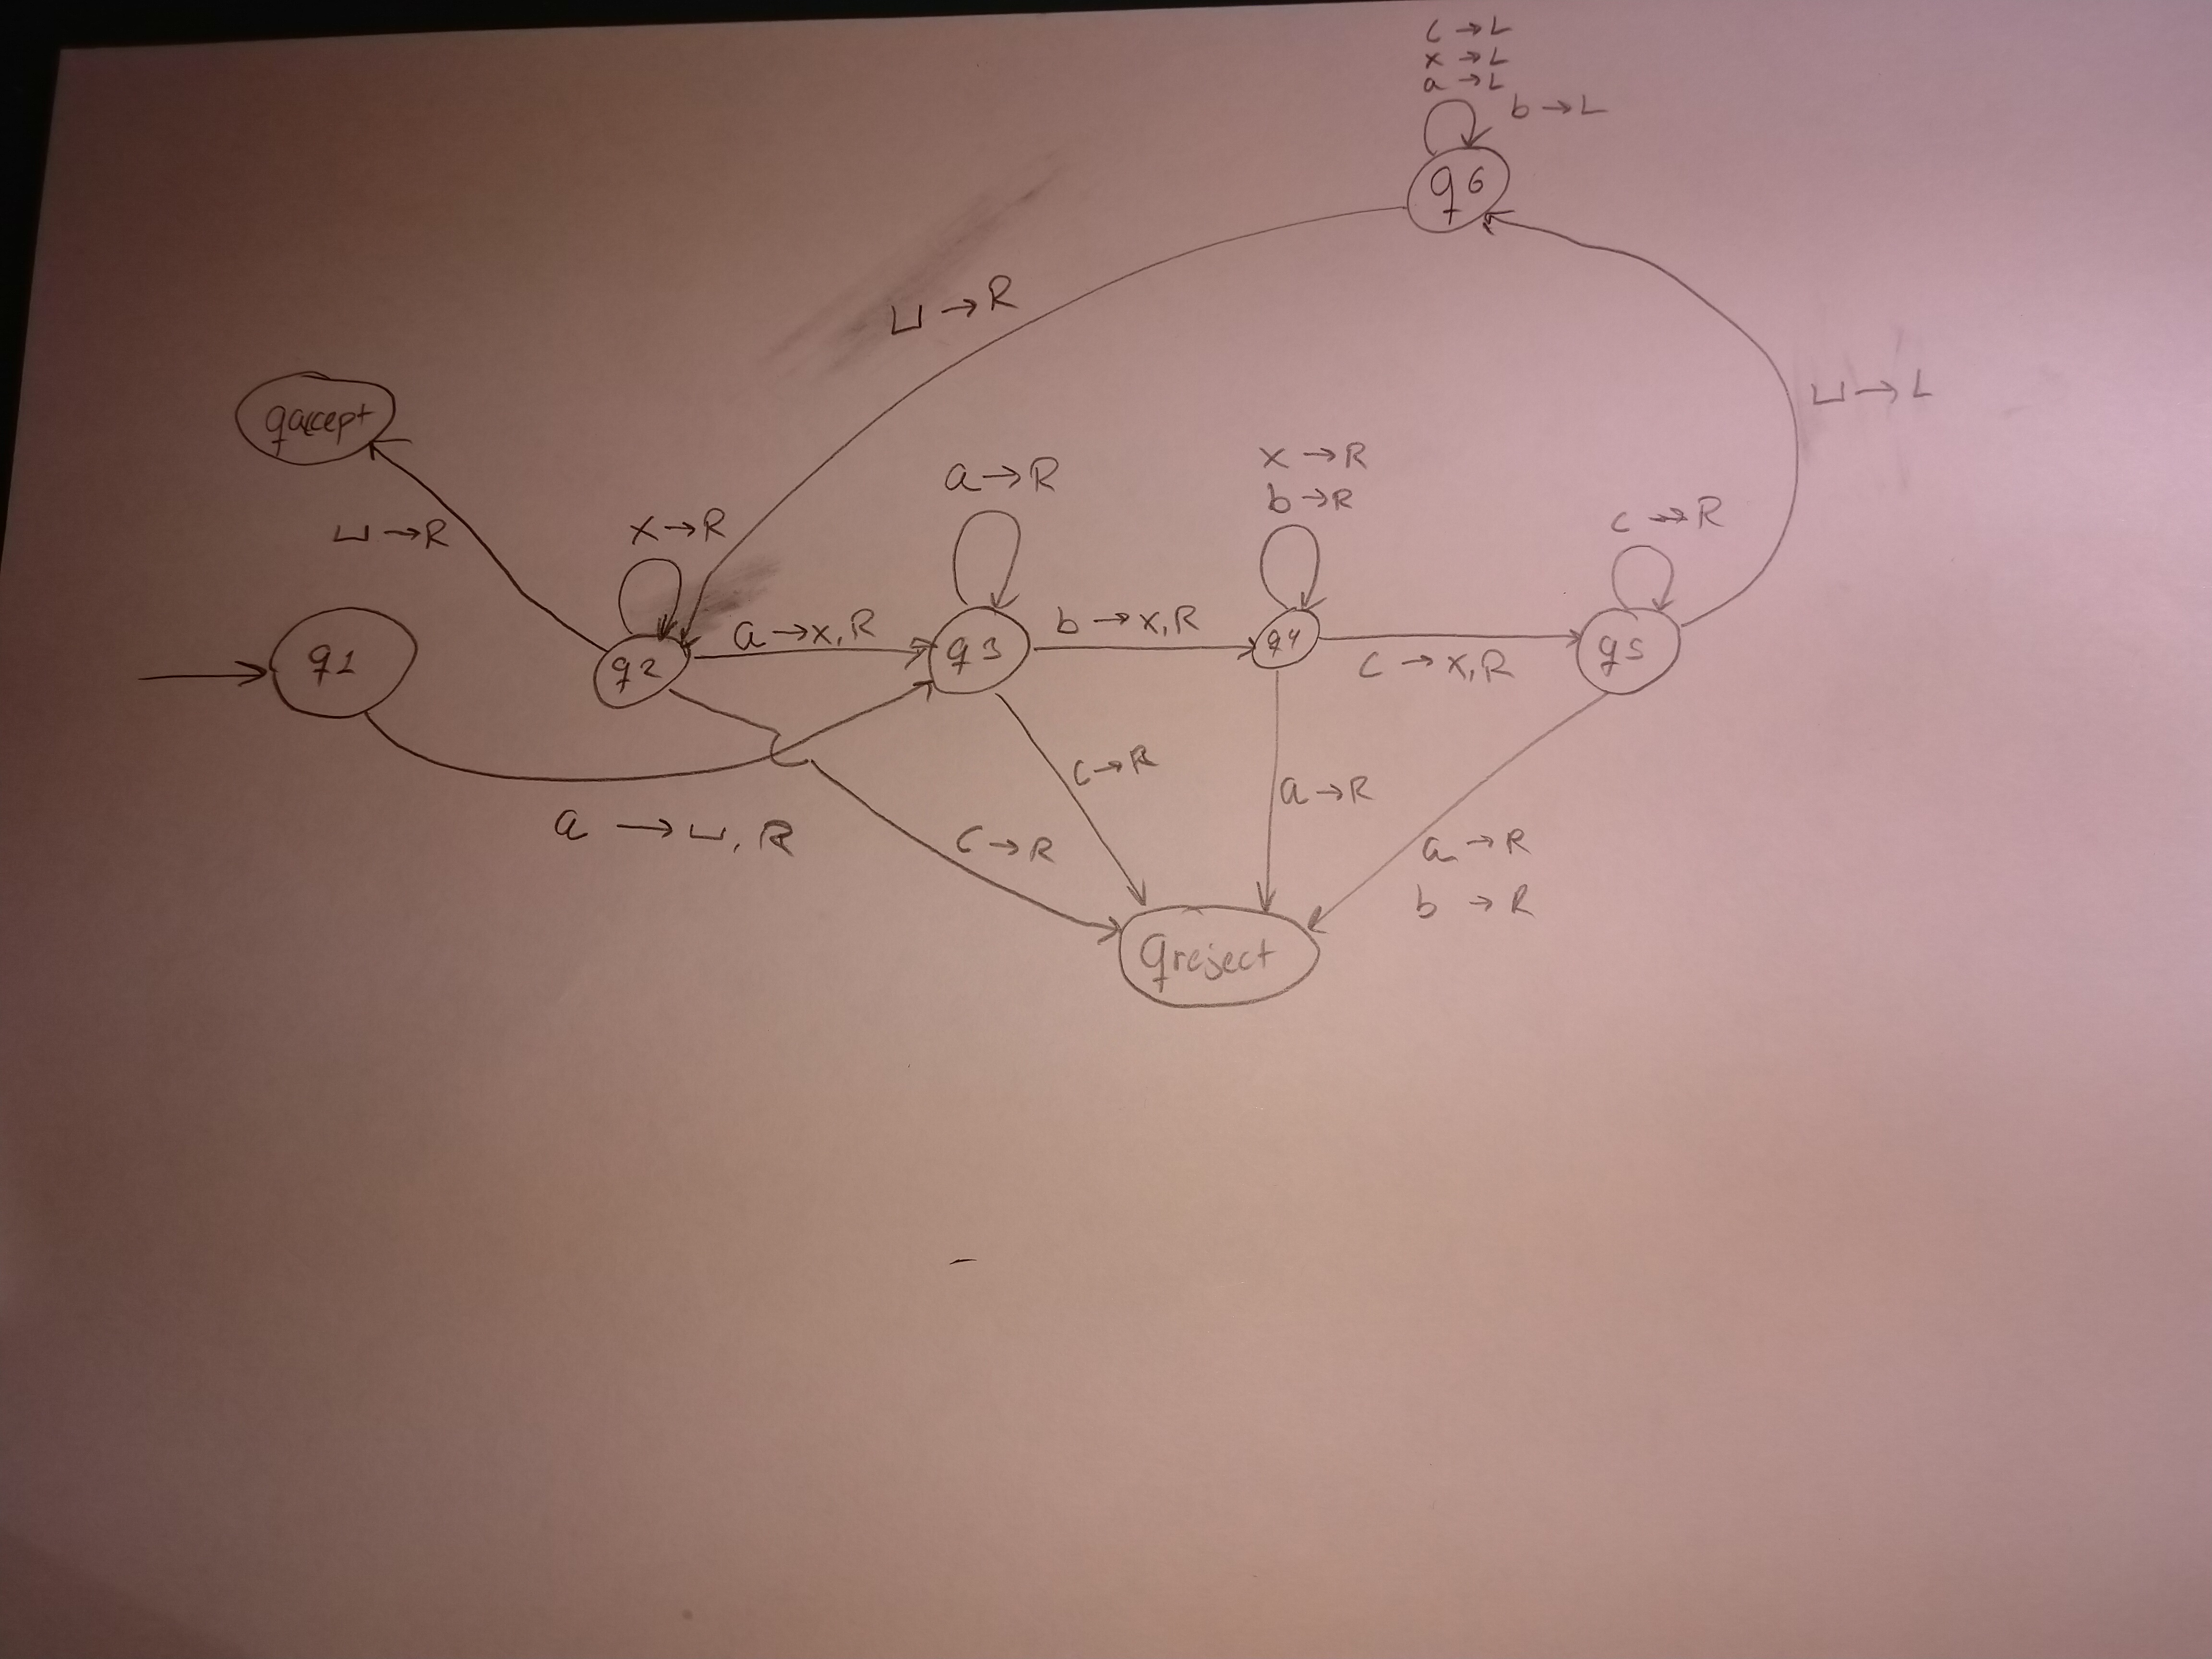
\includegraphics[scale=0.1]{mynd}

\end{document}